Durant mon stage de Master 1, j'ai effectué une mission qui tournait autour d'une problématique simple : donner la possibilité à un utilisateur de décrire une chose et comprendre l'objet de cette chose côté machine. Plus précisément il me fallait catégoriser un texte pour pouvoir ensuite le classifier (parle t-on de science, d'écologie ?, etc.). Quelques pistes m'ont été données pour commencer mes recherches, notamment le traitement du langage naturelle avec les possibilitées liées au web sémantique. C'est en explorant les ambitions du web sémantique que je me suis aperçu des enjeux d'un web ouvert aux données. En formulant des requêtes en langue naturelle ou structurée (type SQL) il est possible de récupérer des données formatées et liées, exploitables par une machine. Avec l'enjouement pour l'intelligence artificielle qui a explosé grâce au big data \cite{sh}, la donnée est devenu précieuse. Beaucoup de problématiques de calcul et d'apprentissage tournent autour de la donnée, dans le machine learning par exemple il faut des données fiables, structurées et en grande quantité. La création de dataset prend du temps et nécessite souvent une intervention externe du fait de la quantité de données à traiter manuellement. Par exemple ClaimBuster (outil que nous présenterons plus tard), a nécessité 3 mois de travail et 226 participants pour créer un dataset viable \cite{hassan2015quest}.
\\*
Pourtant ces données sont disponibles sur le web. N'y aurait-il pas un moyen de réduire ce temps de 3 mois au temps d'une simple requête ?

C'est à une de ces problématiques que le web sémantique (dont nous détaillerons le fonctionnement plus tard) tente aujourd'hui de répondre. Le web sémantique avec l'intégration de la sémantique dans le web vise à donner du sens aux données. Le mot Socrate ne réfère plus à un simple mot mais à un nom, à une personne qui possède une date de naissance, une nationalité, etc. Chaque donnée va référer à un objet qui possède des attributs universels qui le décrivent \cite{schemaPerson}.
\\*
Le web sémantique a déjà eu un impact important sur le web mais méconnu, ce qui peut s'expliquer par le fait qu'il est souvent défini comme un outil fait par des scientifiques pour des scientifiques \cite{semantic_web_has_failed}.
\\*
Un des cas les plus important (et visible) est l'intégration de la sémantique dans le système de recherche de Google. Cela se traduit par des informations organisées à l'écran comme les infoboxes (panel situé à droite qui détaille notre recherche) ou encore des réponses directes aux recherches, exemple : \enquote{Quel est le vrai nom de molière ?} va nous afficher directement la réponse.

Le web sémantique a ouvert toutes sortes de données autour de différents thèmes : la médecine, le e-commerce, etc. La plupart des CMS permettent à leur utilisateurs de structurer leur données et de les ouvrir au reste du monde.
\\*
En médecine on peut noter \href{http://bio2rdf.org/}{Bio2RDF}, projet open source qui regroupe plus de 11 milliards de triples relatifs aux sciences de la vie et à la recherche clinique. On peut aussi citer DBPedia qui est une référence dans le domaine du web sémantique et qui s'est fixé pour but, depuis 2007, de produire des données liées avec des informations extraites de wikipédia.

Toutes ces données sont facilement maniables et interconnectables. Dans le cas présent nous allons voir comment ces données sont utilisées et pourrait être utilisées pour lutter contre la désinformation.

\subsection{La désinformation}

\enquote{La désinformation est un ensemble de techniques de communication visant à tromper des personnes ou l'opinion publique pour protéger des intérêts (privés ou non) et/ou d'influencer l'opinion publique.} \cite{wiki:desinformation}

La désinformation est donc un acte conscient et intentionnel ayant pour but de nuire à un groupe de personnes ou d'orienter son opinion. Elle peut se traduire par de la propagande, du prosélytisme ou de la manipulation sur tout type de sujet. Elle peut prendre tout type de configuration, mais prend souvent la forme d'allégations alarmantes ou révoltantes qui vont frapper le lecteur. Le but est de susciter une émotion forte pour que le lecteur s'empresse de partager l'information. Un mensonge plus frappant qu'une vérité se diffusera plus vite et plus loin avec un impact plus important. On estime par exemple, que sur twitter, une fake news a 70\% de chance en plus d'être partagée qu'une autre information \cite{vosoughi2017rumor}. 
Ainsi la désinformation se traduit plus généralement par une tentative de manipulation de l'opinion publique (exemple \href{https://www.20minutes.fr/societe/2261439-20180426-video-evacuation-tolbiac-retour-naissance-fake-news}{ici}) en transmettant des informations partiellement erronée (il est plus facile de croire à un mensonge enrobé de vérité). 

Il faut tout de même différencier la désinformation politique dont sont à l'origine des grandes organisations ou des états (on parle souvent de propagande) de la désinformation économique qui touche plutôt au buzz et à toute forme de reconnaissance (réseaux sociaux, etc.).

\subsection{Fake news}

Sur internet quand on parle de désinformation, on parle de fake news ou fausses nouvelles. On définit une fake news comme étant une information dont le but est de tromper consciemment un lecteur. Une fake news peut donc être définie comme étant une tentative de désinformation mais qui pour la plupart visent à induire en erreur et créer du buzz autour d'un fait. Elle sont particulièrement présentent sur les réseaux sociaux et dans les usines à clics. Mais on les retrouvent aussi dans la presse spécialisé ou encore dans les médias politisés dont le but est la propagation de fausses informations pour servir leurs intérêts (retouche d'image, etc.).  Mais un article faux n'est pas forcément une fake news tant qu'il n'y a pas l'intention de tromper, l'article peut avoir des fins humoristiques ou satiriques par exemple.

Une information se base sur un fait réel et donc vérifiable. Afin d'identifier une information comme étant fausse il faut pouvoir le prouver factuellement. Il est donc important de connaître l'existant (un ensemble d'informations vraies) pour pouvoir identifier une information fausse. Ici le but n'est pas de lutter contre ou éradiquer les fake news (cela reste de la liberté d'expression, dans une certaine mesure). Nous chercherons simplement à les identifier.

\paragraph{Contexte}

Même si le phénomène des fake news existe depuis longtemps, ce n'est que récemment, avec la campagne présidentielle américaine de 2016 et l'ingérence russe, qu'il a pris de l'ampleur. C'est à ce moment que l'on s'est vraiment rendu compte que toutes ces informations qui circulent sur internet ont un impact important sur le monde. Par exemple, en juillet 2016, le site wtoe5news a rapporté que le pape François avait approuvé la candidature à la présidence de Donald Trump. Cette information a été partagée plus d'un million de fois sur Facebook. A aucun moment il n'est mentionné le fait que wtoe5news est en fait un site d'informations satiriques. Ces fausses nouvelles se sont propagées au travers des sites d'informations et des réseaux sociaux, notamment Google, Twitter et Facebook. La tendance des utilisateurs à se servir des réseaux sociaux comme source d'information fait que n'importe qui s'improvise journaliste. Et qui s'improvise journaliste peut s'improviser propagandiste. En 2016, 62\% des adultes résidants aux États-Unis utilisent au moins parfois les réseaux sociaux pour s'informer. Malgré les retombées médiatiques suite à l'ingérence russe, ils sont 67\% en 2017 \cite{news_across_platforms_2017}.

Il est important de savoir quel impact peut avoir une fausse information lorsqu'elle est vu par des millions de personnes. Durant l'élection, une personne a été confronté en moyenne à 3 fake news qui ont pu altérer son jugement \cite{allcott2017social}. De plus il est démontré que cette exposition à la désinformation a en partie influencé les résultats de l'élection présidentielle. Les fake news les plus partagées favorisaient l'élection de Trump. En moyenne une campagne de télévision à un impact de 0.02\% sur les votes d'une élection \cite{spenkuch2016political}. Si une fake news est aussi persuasive qu'une campagne de télévision on peut clairement dire que les fake news ont joué un rôle, déterminant ou non, dans l'élection de Trump.

\paragraph{Pourquoi favoriser leur détection ?} A cause de l'impact sur le monde réel que cela peut avoir. Susciter une vive émotion dans l'opinion publique est une des finalités de la fake news. Cela peut avoir des conséquences graves sur les évènements qui se déroulent (réponse par la violence, la haine). C'est un constat encore plus vrai en temps de guerre ou durant des périodes sensibles.

\paragraph{Initiatives contre les fake news}

Le combat contre les fake news se déroule principalement sur les plateformes concernées.  https://www.engadget.com/2018/03/29/facebook-stepping-up-fight-fake-news/?guccounter=1

Que fait-on dans le monde réel pour lutter contre les fakenews ?
Survey of initiatives against fake news : \cite{haciyakupoglu2018countering}

\todo{parler de facebook/google }

\subsection{Fake news et intelligence artificielle}

Comment l'intelligence artificielle peut-elle aider à la détection automatique de fake news ? 

Il existe différents outils qui intègre de l'intelligence artificielle dans leur système pour agir sur les différentes étapes de la détection d'une fake news. Nous allons commencer par définir un processus simple d'évaluation de la véracité d'une fake news (voir Figure \ref{fake_news_process}).

\begin{figure}[ht]
\centering
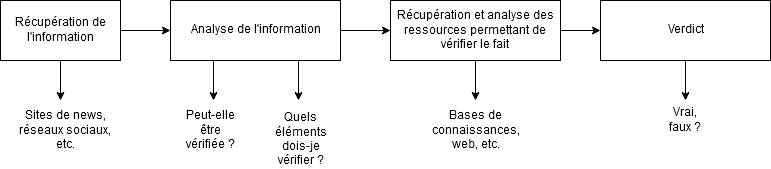
\includegraphics[width=\textwidth, draft=false]{diagrams/fake_news_process.png}
\caption{Processus de détection d'une fake news}
\label{fake_news_process}
\end{figure}

L'analyse du fait à vérifier et des ressources permettant de le vérifier, sont des étapes qui font appellent aux techniques d'apprentissage de la langue mais aussi de la machine. Des solutions hybrides existent et permettent d'étendre le traitement de la langue en y ajoutant une dimension plus factuelle et réelle \cite{conroy2015automatic}.

Pour analyser un fait, nous avons une approche qui se repose sur le traitement automatique du langage naturel (TALN). Le but de cette approche est d'analyser le texte brut pour identifier des patterns qui montre qu'un texte est trompeur. Lorsque le langage est trop négatif ou laisse transparaître des émotions trop vive. Lorsque les mots utilisés sont similaires à ceux utilisés dans de précédentes analyses positives. Ces variations du discours ont conduits des travaux qui ont permis d'analyser les changements linguistique d'un discours lorsque celui-ci est faux \cite{markowitz2014linguistic}. Le langage a tendance à être plus superficiel, moins descriptif, moins complexe etc. Beaucoup d'indices permettent d'établir un verdict. 
\\*
Cette approche est en revanche trop peu déterminante et trop peu certaine. Elle est utilisée principalement pour complémentariser des approches plus sophistiquées. En effet Pour détecter et prédire la tromperie il est nécessaire d'utiliser des structures syntaxiques plus avancées. L'analyse syntaxique profonde (deep syntax) va permettre de construire des ensembles de règles permettant de décrire la structure syntaxique d'un texte. Appliqués à un texte, ces ensembles de règles vont permettre d'identifier des patterns plus évolués permettant une détection plus précise et certaine des cas de tromperie \cite{feng2012syntactic} \cite{collinsprobabilistic}.

Les méthodes d'analyses linguistiques sont innombrables et s'intéressent toutes à identifier des patterns différents. Il s'agit plus de détecter le mensonge que de le prouver. Il est donc nécessaire de coupler ces approches avec des méthodes qui vont prouver factuellement que le fait est vrai ou faux.

C'est ici que le web sémantique va jouer un rôle prépondérant. Les bases de connaissances (ou Knowledge Base, abrégé KB) vont apporter un contexte sémantique aux données. Une KB va représenter le monde en attribuant aux données des propriétés qui vont la décrire. Ainsi lorsque je veux savoir si Barack Obama est allé à Harvard, je vais étudier les relations qui existent dans ma base entre l'entité Barack Obama et Harvard pour établir un verdict. Nous verrons en détail des méthodes qui utilisent cette approche dans la section \ref{section_knowledge_graph}.

Le machine learning est aussi une approche viable. L'outil de fact-checking ClaimBuster par exemple va utiliser le machine learning pour identifier des patterns de phrases pouvant contenir des faits à vérifier. Cela permet d'identifier dans un texte les phrases qui nécessitent une vérification. 
\\*
On a aussi des moyens plus complémentaires comme la simple vérification de la source émettrice de l'information (ce qui aurait pu empêcher la propagation de la fake news sur l'implication du pape dans la campagne  de Donald Trump). Il est aussi possible d'établir un score de confiance sur les sources d'information en fonction des expériences passées : ce sont souvent les mêmes sources qui propagent de fausses informations.
\\*
D'autres part, l'analyse des médias utilisés dans un article peut conduire à détecter de potentiels cas de fake news : si un article de 2017 présente des images d'une manifestation violente, on va rechercher des informations sur ces images. Sur google image il est possible d'effectuer une recherche par image et ainsi déterminer la date de la première apparition d'une image sur le web. Si une image datant de 2012 se retrouve sur un article de 2017, alors c'est une possible tentative de désinformation (exemple \href{https://www.lemonde.fr/les-decodeurs/article/2017/10/02/violences-policieres-en-catalogne-attention-aux-images-trompeuses_5194905_4355770.html}{ici}). Il est aussi possible de déterminer si une image a été altérée et retouchée \cite{krawetz2007picture}.

L'intelligence artificielle a un rôle prépondérant a jouer dans la détection de fake news. Elle intervient à toutes les étapes. Principalement dans le TALN mais aussi dans la façon de traiter l'information (machine learning).

Pour conclure, nous avons vu que les méthodes liées à l'analyse syntaxique vont se construire autour du TALN et de modèles statistiques tandis que celles sur les KBs vont regrouper des méthodes orientées sur la théorie des graphes. Mais ces deux approches sont complémentaires. L'analyse syntaxique va permettre à la KB d'identifier les données qu'elle manipule et de les structurer. Inversement la KB va permettre à l'analyse syntaxique d'ajouter une dimension concrète et matérielle aux données. Et permettre ainsi de replacer la donnée dans l'existant. D'autres méthodes permettent d'étendre ces approches et s'avèrent essentielles pour un système de fact checking autonome (si un article est vrai mais présente des images trompeuses, il est nécessaire de s'en rendre compte).

On discerne donc ici deux approches, l'une qui va tenter d'analyser le fait énoncé et rechercher un argumentaire sur le web en appliquant des algorithmes de TALN pour construire un verdict. Et l'autre qui va se baser sur des données issues du web, déjà structurées et formatées, pour établir son verdict.

\subsection{Fact-checking}

Le fact-checking ou vérification de faits représente l'acte de vérifier la véracité d'une assertion. Il s'agit de traiter l'information afin de démêler le vrai du faux, du partiellement vrai du partiellement faux. Il est apparu aux États Unis dans les années 2000. Le fact checking est considéré aujourd'hui comme une forme de journalisme à part entière \cite{lemonde_fact_check_nouveaute_journalistique}. Avec la montée des réseaux sociaux et de la propagation toujours plus rapide de et massive l'information, le fact checking a pris de l'ampleur récemment. De plus en plus de site d'informations se munissent de leurs propres laboratoires de fact checking \cite{memoire_fact_check_nouveaute_journalistique}. 

Seulement les sources d'informations sont innombrables et le flux de données journalier est tel qu'il est impossible de vérifier chaque information manuellement. Que ce soit sur des blogs, les réseaux sociaux, les sites d'information, etc. filtrer l'information et la vérifier représente un temps de travail important. Les sites peuvent apporter leur propre système de fact checking humain (voir \href{http://decodeurs.blog.lemonde.fr/}{ici}) mais le nombre de faits couverts reste très limité.

\paragraph{Fact-checking : les limites}

Le fact-checking est un travail qui est chronophage, en effet il faut tout d'abord trouver et identifier les faits vérifiable et dignes d'intérêt. Il y a ensuite un travail de recherche pour comprendre le fait et le vérifier en faisant attention de ne pas tomber soi-même dans le piège de la désinformation. Cela signifie confronter et vérifier ses sources. 
Tous ces critères font qu'entre le moment ou une déclaration est faite, et celui ou elle est vérifiée s'écoule un certain laps de temps, qui peut éventuellement rendre le fact-checking inutile si la déclaration a déjà eu l'impact voulu.

\paragraph{Quels objectifs ?}

L'objectif derrière le fact checking reste actuellement très politique, il s'agit de traquer les mensonges de personnalités influentes.

Mais à terme le fact checking doit permettre de toujours manipuler une information avérée et sûre quelque soit sa source ou sa forme.

Il n'existe actuellement aucun système universel, 100\% automatisé et 100\% fiable qui permettent de réaliser des opérations de fact-checking sur tout type de support. La finalité d'un système de fact-checking serait tout d'abord d'être capable de caractériser, classifier et comprendre l'information pour ensuite vérifier sa légitimité. 

\paragraph{Système entièrement autonome ou du moins le plus possible}

Quelle serait les tâches d'un système entièrement autonome ? Quelle est la faisabilité de chacune de ces tâches ? Et enfin quelle marge d'erreur est on prêt à accepter avant de définir notre système comme entièrement autonome ? Enfin, confier à un système informatique autonome la responsabilité de vérifier des faits revient à demander à une machine de faire du journalisme. Cela peut poser des problèmes éthiques, peut-on faire confiance à une machine pour nous dire ce qui est vrai ou faux ?

Un tel système doit pouvoir extraire une assertion d'une source et la vérifier sans intervention humaine et dans un temps raisonnable. Pour cela il doit pouvoir se "nourir" de différentes sources d'informations qu'il va confronter. Plusieurs challenges importants entre en compte dans le vérification d'un fait.

\paragraph{Challenges}

Comme nous l'avons précisé pour qu'un fait soit analysé il faut tout d'abord qu'il soit compris. Il faut donc faire comprendre au système le langage humain, c'est ce qu'on appel le traitement automatique du langage naturel (TALN). C'est un domaine vaste qui fait appel à de nombreux sous domaine dans le traitement du langage comme l'analyse syntaxique ou l'analyse sémantique. Bien que très avancée, cette science est en revanche loin d'être parfaite \cite{nlp_not_perfect}.

Mais un système aussi performant soit-il ne fonctionnera pas sans données fiables. Il faut pouvoir trouver et collecter ces données pour alimenter le système. Les sources de données structurées et utilisables sont innombrables, que ce soit avec le développement du web sémantique, du linked-data, des bases de connaissances, des apis de type REST (Wikimédia) et de l'open data on possède déjà des sources de données conséquentes et fiables. On a ensuite des sources de données plus générique, moins ordonnées mais tout aussi exploitable. Je parle ici des sites d'information et plus généralement de toutes les informations disponibles sur internet : réseaux sociaux, etc. Ce sont des sources de données plus ou moins fiable mais la quantité d'information produite par ces sources est considérable. Ces sources peuvent être interrogées via des outils de type web scraping et data mining.
Toutes ces sources de données peuvent être confrontées pour permettre de chercher et étoffer un fait pour pouvoir le comprendre et le vérifier.
Mais les sources de données ne se limitent pas à ce que l'on trouve sur internet.

On identifie donc 3 sources de données différentes, les données : 

\begin{itemize}
    \item Déjà traitées par des sites spécialisés ou communautaires : beaucoup de sites d'information ont développés leurs propres systèmes de fact-checking (tous manuels). 
    \item Structurées ou semi-structurées : issues de l'open data, ou d'api telles que wikimédia
    \item Non-structurées : issues de toutes sources potentiellement utilisables
\end{itemize}

Les données non structurées peuvent se trouver directement dans la vie réelle à travers différents médias : les chaînes de télévision, les émissions de radio (mais aussi les journaux, magazines), etc. Tout signal vidéo ou audio est potentiellement une source intéressante pour le système. Il faut pouvoir interroger et structurer ces sources : savoir qui parle, dans quel contexte.

Une fois ces informations structurées nous devons savoir lesquelles définissent des faits réels et vérifiable. Filtrer les informations en fonction de la vérifiabilité d'une assertion. C'est-à-dire éliminer toute phrase qui définit une opinion, de l'humour, de l'ironie, figures de style, etc. et bien sûr les phrases lambda. De plus comment détecter qu'un fait se construit sur plusieurs phrases ? Comment construire une argumentaire appuyé par des preuves concrète qui permette de remettre en cause le fait.

\subsection{Objectifs}

\todo{But du mémoire : voir l'ensemble des techniques viable et proposer un système cohérent reprenant les atouts de chaque méthodes/concept + architecture technique}

J'ai choisi ce sujet car il fait appel à des technologies et des domaines de recherches très nombreux que j'ai souvent survolé : web sémantique et linked-data, analyse sémantique, bases de connaissances, traitement automatique du langage, machine learning, knowledge graph, web scraping, web crawling, data mining, etc. 
\\*
En voulant analyser l'information de façon automatique on cherche ici à cartographier et comprendre les ressources disponibles sur le web. Analyser toutes les données disponibles pour en comprendre le sens, et construire des modèles cohérents permettant de structurer l'information pour élaborer des modules basés sur des algorithmes d'apprentissage efficaces. C'est-à-dire récupérer des informations, les structurer et construire des algorithmes issus de ces données par apprentissage supervisé. La finalité de ces algorithmes est multiple : détection de fake news, détection d'image, etc. Ce que je veux montrer ici c'est l'enjeu derrière un web structuré : je souhaite obtenir un dataset d'images me permettant d'entraîner mon algorithme de détection de visage ? Je n'ai qu'une simple requête à faire. C'est tout à fait possible sur des bases de données de type \href{https://fr.wikipedia.org/wiki/Triplestore}{Triplestore} \cite{wiki:Triplestore} qui vont organiser la donnée comme un graphe connecté ou chaque noeud est relié par une relation. C'est un objectif très vaste voir impossible (\todo{citation sur les détracteurs du web sémantique}). Mais pour lutter contre la désinformation et arriver à un système de fact checking efficace et autonome c'est un prérequis important.

\todo{Faire évoluer le but du mémoire en fonction des résultats}
Le but de ce mémoire est d'étudier différentes approches utilisées dans le fact checking automatique pour pouvoir proposer un système viable et cohérent. Nous tenterons de construire un système reprenant les atouts de chaque méthodes et concepts afin de proposer une architecture technique qui tente de répondre à plusieurs problématiques rencontrées par les systèmes existants.

\todo{Plutôt que d'essayer de vérifier la véracité d'un fait pourquoi ne pas collecter des infos autour de ce fait, construire un argumentaire et laisser l'utilisateur être seul juge ?}